
\section{Multi-log results}
\label{sec:multilog}

\label{sec:denominator}
Every point estimate in this section comes from one master surface ---
one file, named in the code-availability statement --- computed by one pass of
one pipeline over
\nPairs\ log--target pairs, \nLearners\ learners, \nSplits\ splits, \nQuality\
register-quality conditions, the nested baseline ladder and \nMetrics\
instruments including the \nGrid-point decision-curve grid. Its
\nSurfaceRows\ rows \emph{include} the intercept-only rung, so that the
surface is complete; no admissible set contains it, and the
\nDeclaredAdmissibleScalar\ admissible scalar cells every headline is computed
on exclude it. Every interval is the basic construction of
Section~\ref{sec:boot} and every band the whole-surface simultaneous
construction of Section~\ref{sec:simbands}, and each table names which it
prints. The denominator audit is in Table~\ref{tab:denominator}: declared
equals computed on all \nPairs\ pairs, with \nDuplicateCells\ duplicates and
\nMissingCells\ missing, and the inference surface (\nInferenceScalar\ scalar
members) is a subset of it cell for cell, which \texttt{verify\_numbers}
asserts.

\subsection{The master table}

\begin{table}[t]
\centering
\small
\resizebox{\ifdim\width>\linewidth\linewidth\else\width\fi}{!}{%%
\begin{tabular}{llrrrlrr}
\toprule
log & target & V at reference & lo & hi & region & rho & misreport rate \\
\midrule
BPIC13\_closed & handover & -0.009 & -0.041 & 0.018 & conditionally harmful & -0.033 & 0.428 \\
BPIC13\_incidents & duration & 0.028 & 0.014 & 0.056 & conditionally beneficial & 0.533 & 0.393 \\
BPIC13\_incidents & handover & 0.037 & 0.027 & 0.051 & conditionally beneficial & 0.867 & 0.111 \\
BPIC14 & duration & 0.096 & 0.090 & 0.109 & conditionally beneficial & 0.781 & 0.205 \\
BPIC14 & handover & 0.167 & 0.146 & 0.204 & sign-changing & 0.541 & 0.340 \\
BPIC15\_1 & duration & 0.001 & -0.030 & 0.045 & conditionally beneficial & 0.200 & 0.500 \\
BPIC15\_1 & handover & 0.007 & -0.008 & 0.021 & conditionally beneficial & 0.033 & 0.242 \\
BPIC15\_3 & duration & 0.035 & -0.004 & 0.067 & conditionally beneficial & 0.500 & 0.191 \\
BPIC15\_3 & handover & -0.003 & -0.048 & 0.061 & unresolved & 0.000 & 0.577 \\
BPIC15\_4 & duration & 0.035 & 0.010 & 0.078 & conditionally beneficial & 0.033 & 0.500 \\
BPIC15\_4 & handover & 0.001 & -0.028 & 0.056 & unresolved & 0.000 & 0.422 \\
BPIC15\_5 & duration & 0.032 & -0.024 & 0.090 & conditionally beneficial & 0.267 & 0.385 \\
BPIC17 & duration & 0.002 & -0.003 & 0.012 & conditionally beneficial & 0.200 & 0.353 \\
BPIC19 & duration & 0.024 & 0.011 & 0.042 & sign-changing & -0.367 & 0.349 \\
Helpdesk & duration & -0.020 & -0.043 & -0.002 & conditionally beneficial & 0.033 & 0.257 \\
RoadFines & duration & 0.031 & 0.024 & 0.037 & sign-changing & 0.400 & 0.136 \\
Sepsis & duration & 0.153 & 0.108 & 0.207 & uniformly beneficial & 1.000 & 0.056 \\
UCI498 & duration & -0.007 & -0.010 & 0.007 & conditionally beneficial & 0.133 & 0.502 \\
UCI498 & handover & -0.003 & -0.007 & -0.001 & sign-changing & 0.233 & 0.506 \\
\bottomrule
\end{tabular}%
}
\caption{The master table. One row per admitted log--target pair: the increment at the reference specification with its 95\% interval from the nested bootstrap, the resolution region, the robustness index $\rho$, and the share of admissible specifications whose sign disagrees with a conventional one-number report. The reference cell's sign and the region need not agree, and on several pairs they do not: a surface can be conditionally beneficial while the one cell an analyst would have stood on is negative, which is this paper's argument in a line.}
\label{tab:master}
\end{table}


Table~\ref{tab:master} is the frozen master table: one row per log--target
pair, the increment at the reference specification with its simultaneous band,
the region label, the robustness index and the sign-disagreement rate of a
conventional one-number report. The reference specification is declared and is
the same everywhere --- one-hot logistic regression, the single temporal
holdout, the clean register, the intake block plus the free field as the
baseline, ROC AUC --- and its region and $\rho$ columns are the
ones Section~\ref{sec:regions} reports while its
sign-disagreement column is the all-cells rate of Table~\ref{tab:misreport}
under the equal-level measure. The reference cell's sign and the
region label need not agree, and on several pairs they do not: a surface can
be conditionally beneficial while the one cell an analyst would have stood on
is negative, because the label ranges over the whole inference family and the
reference cell is one member of it. Table~\ref{tab:triple} prints the counts
each label rests on, and Table~\ref{tab:roles} which attribute plays the
register on each row.

\subsection{What the choices are worth}
\label{sec:axes2}


\begin{figure}[t]
\centering
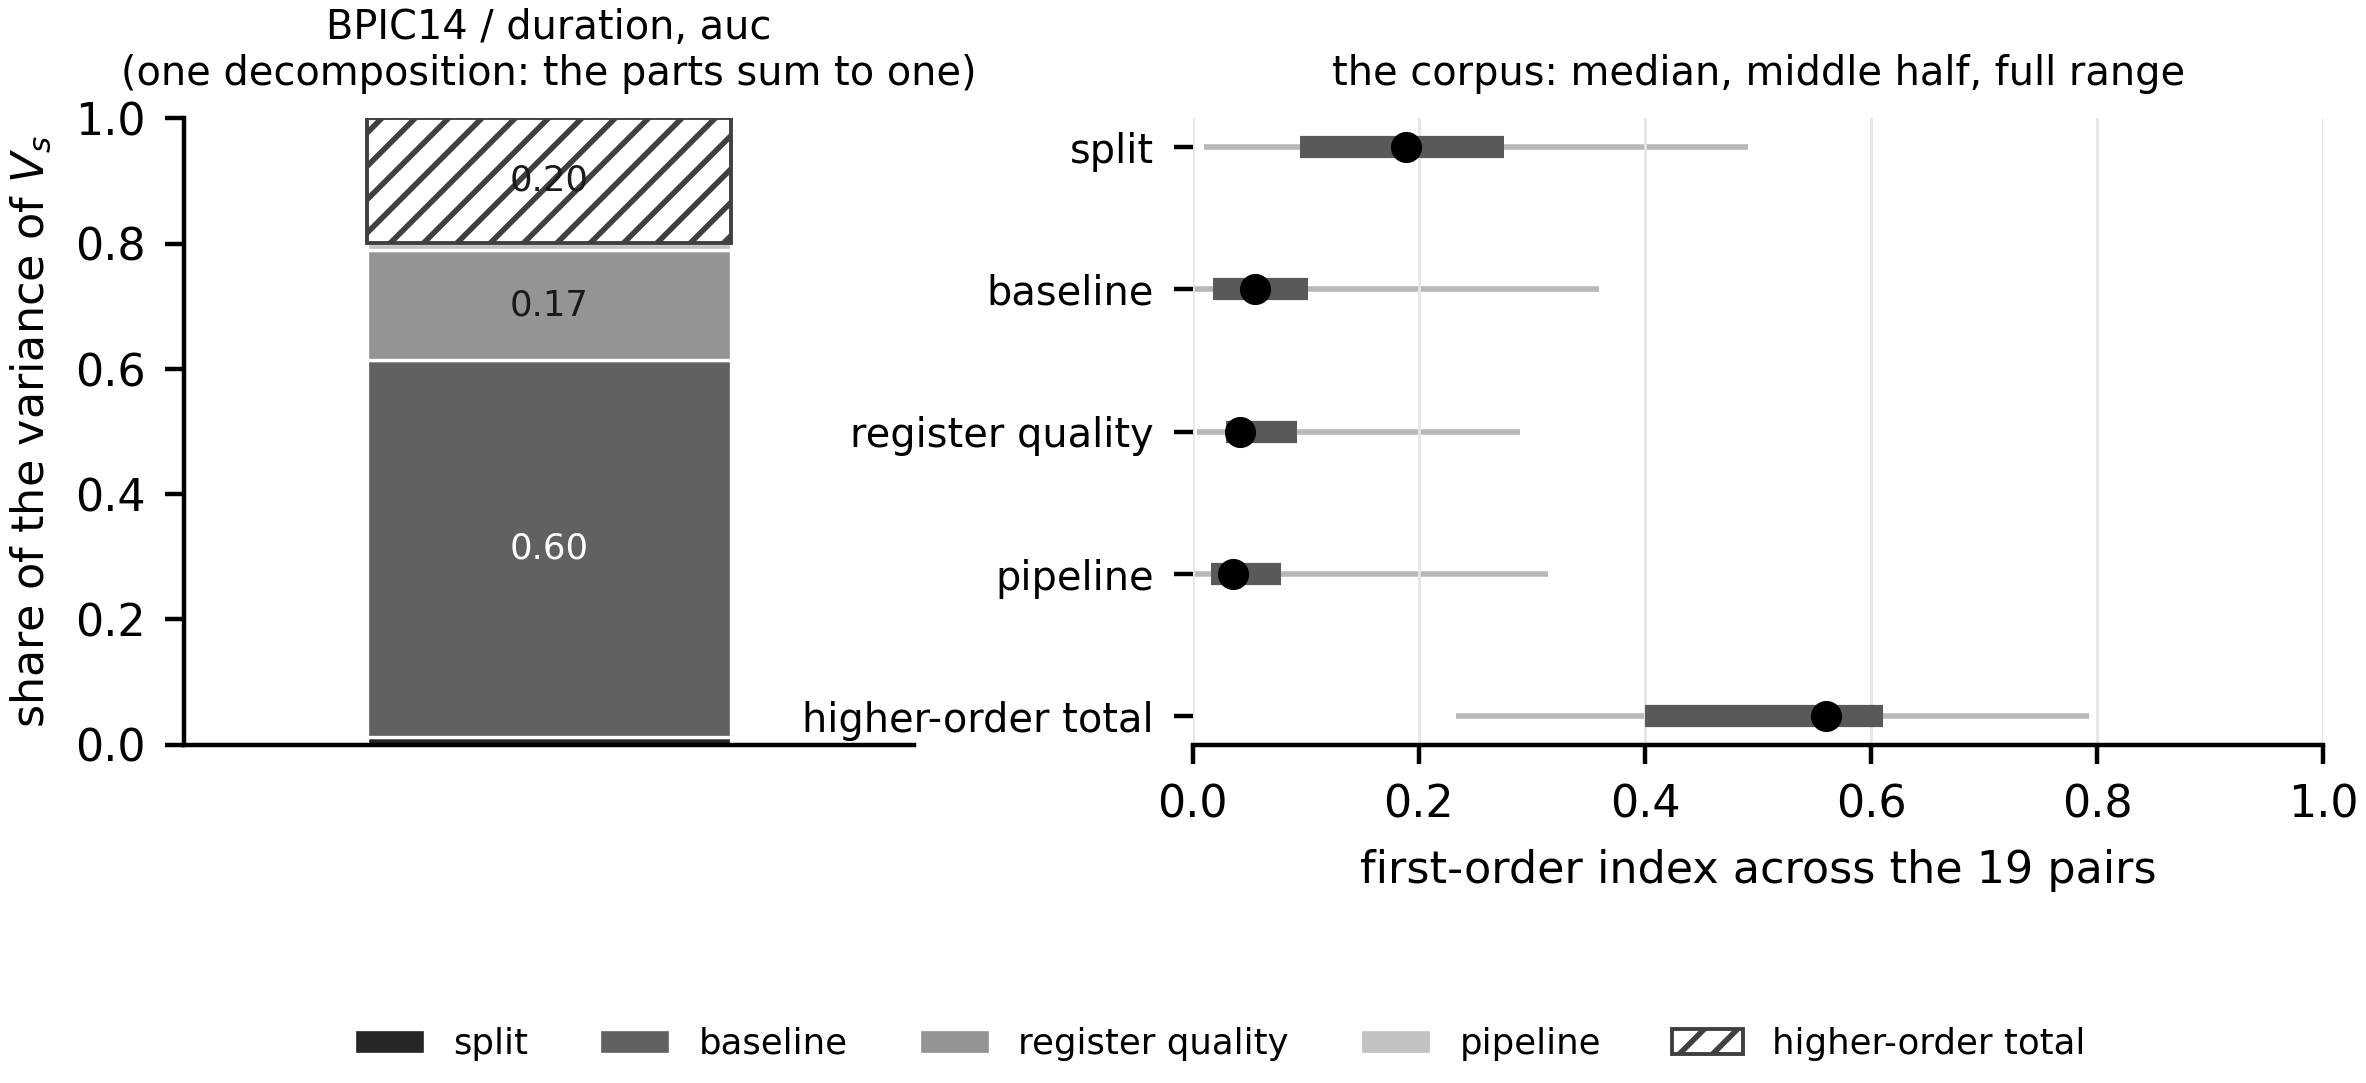
\includegraphics[width=\linewidth]{figS2_sobol.png}
\caption{The decomposition, within instrument, under the equal-level measure.
\emph{Left}: one pair at one instrument, so the components are a
decomposition and the parts sum to one exactly --- the largest pair in the
corpus, at the reference instrument, which is the cell every other table
reports at. The hatched segment is the total higher-order share
$1 - \sum_i S_i$ of~\eqref{eq:inttotal}. \emph{Right}: each axis's
first-order index across the corpus, as the median over pairs with the range
the middle half occupies and the full range. Nothing on the right is stacked,
because a median over pairs and a median over instruments do not add and a
stacked bar of them would invite the addition.}
\label{fig:sobol}
\end{figure}

Table~\ref{tab:sobol} and Figure~\ref{fig:sobol} give the decomposition,
computed within each instrument in that instrument's own units, under the
equal-level measure. The table's first four columns are, per pair, the median
over the five instruments of each axis's first-order index; its last column is
the largest per-axis interaction \emph{involvement}. Three aggregations of
this table are quoted below and they are not interchangeable, so each is named
where it appears: the median over pairs of a column of this table; the
\largestFirstOrderPct\ figure, which is the median over pairs of the median
over instruments of the \emph{per-instrument} largest first-order index, and
which is therefore not obtainable by taking a maximum across the four printed
columns; and the corpus medians of the higher-order share. The per-instrument
quantities the second is built from are in Table~\ref{tab:measures}.

\begin{table}[t]
\centering
\small
\resizebox{\ifdim\width>\linewidth\linewidth\else\width\fi}{!}{%%
\begin{tabular}{llllll}
\toprule
log & target & analyst choice & counterfactual & mixed & resampling \\
\midrule
BPIC13\_closed & handover & 31.5 & 2.9 & 5.8 & 59.8 \\
BPIC13\_incidents & duration & 13.3 & 2.9 & 3.0 & 79.6 \\
BPIC13\_incidents & handover & 19.2 & 9.9 & 4.5 & 42.3 \\
BPIC14 & duration & 71.9 & 15.1 & 7.9 & 5.1 \\
BPIC14 & handover & 73.9 & 12.7 & 10.3 & 3.6 \\
BPIC15\_1 & duration & 9.4 & 3.9 & 4.7 & 80.5 \\
BPIC15\_1 & handover & 13.4 & 3.6 & 3.6 & 62.6 \\
BPIC15\_3 & duration & 11.7 & 8.1 & 1.5 & 77.6 \\
BPIC15\_3 & handover & 22.3 & 0.4 & 2.5 & 76.1 \\
BPIC15\_4 & duration & 11.3 & 2.5 & 5.6 & 81.6 \\
BPIC15\_4 & handover & 12.4 & 3.1 & 5.7 & 71.7 \\
BPIC15\_5 & duration & 17.4 & 4.2 & 3.9 & 69.9 \\
BPIC17 & duration & 4.2 & 6.2 & 5.2 & 84.1 \\
BPIC19 & duration & 3.8 & 1.1 & 2.8 & 90.9 \\
Helpdesk & duration & 31.7 & 8.6 & 1.7 & 53.6 \\
RoadFines & duration & 7.0 & 28.9 & 2.1 & 61.7 \\
Sepsis & duration & 13.2 & 14.5 & 5.0 & 71.9 \\
UCI498 & duration & 11.0 & 3.0 & 4.3 & 81.1 \\
UCI498 & handover & 41.0 & 7.1 & 9.3 & 42.4 \\
\bottomrule
\end{tabular}%
}
\caption{THE DECOMPOSITION WITH THE SPLIT AS AN ERROR STRATUM. Per cent of the pooled variance of $V_s$, per pair, median over the \nInstruments\ instruments, under the equal-level measure. The four columns are an exact partition of the orthogonal decomposition's components, and on \emph{each} of the \nDecompositions\ decompositions they sum to 100 to within \stratumPartitionError. \textbf{The printed rows are medians over instruments and therefore need not sum to 100}, for the same reason Figure~\ref{fig:sobol}'s right panel is not stacked: a median is not linear. `analyst choice' collects every component built only from the pipeline and the baseline rung, `counterfactual' the register-quality main effect, `mixed' the components that join the two, and `resampling' every component involving the split --- five of whose six levels are expanding-origin folds on the same data. Dropping the sixth, the single temporal holdout, so that the axis is folds and nothing else, moves the last column's corpus median from \shareResamplingStratumPct\ to \shareResamplingRollingPct.}
\label{tab:strata}
\end{table}


\textbf{Most of what the pooled surface varies over is not specification at
all.} Table~\ref{tab:strata} partitions the decomposition by
\eqref{eq:strata}, exactly and on every decomposition separately. Taking each
column's median across the corpus --- \emph{four medians, which do not add,
and are not four parts of one pair} --- the components involving the split
carry \shareResamplingStratumPct\ of the variance, against
\shareAnalystStratumPct\ for the choices an analyst makes,
\shareCounterfactualStratumPct\ for the register-quality counterfactual and
\shareMixedStratumPct\ for the components that join them. Resampling is the
largest of the four on \nResamplingLargest\ of the \nPairs\ pairs. Dropping
the one split level that is a genuine analyst choice --- the single temporal
holdout, leaving five folds of one rule --- moves that share only from
\shareResamplingStratumPct\ to \shareResamplingRollingPct, so the stratum is
not an artefact of mixing a rule with its folds. The two exceptions
are the case study's own pairs, where the analyst axes carry the richest
grids in the corpus --- \nPipelineLevelsCase\ pipelines and
\nQualityFigOne\ register-quality conditions, against at most
\nPipelineLevelsLarge\ and \nQualityLevelsOther\ on every other pair
(Table~\ref{tab:roles}) --- and the ordering reverses.

\textbf{Net of resampling, no single axis dominates --- and this is a weaker
statement than the pooled surface makes it look.} On the fold-averaged
surface, which carries \foldVarRatioPct\ of the pooled variance, the median
first-order index is \foldSRungPct\ for the baseline rung, \foldSQualityPct\
for the register-quality condition and \foldSPipelinePct\ for the pipeline,
and at the median pair the largest first-order index \emph{within an
instrument} is \foldLargestFirstOrderPct\ --- a median over pairs of a median
over instruments of the per-instrument largest, and so not the largest of the
three medians just quoted. The total higher-order share is
\foldInteractionTotalPct\ once resampling is removed, against
\pooledInteractionMedianPct\ on the pooled surface, and it no longer exceeds
the largest first-order index: pooled, the interactions carry more than any
main effect on \nPooledInteractionExceeds\ of \nPairs\ pairs; net of
resampling, on \nFoldInteractionExceeds. \emph{Most of the variance belongs to
no single axis} is a property of a surface that counts five folds as five
specifications, and it does not survive treating them as what they are. What
does survive is the weaker and still sufficient claim: which axis leads is a
property of the pair --- the rung on \nFoldLeadPairsRung, the register-quality
condition on \nFoldLeadPairsQuality\ and the pipeline on
\nFoldLeadPairsPipeline\ --- so an analyst cannot learn from somebody else's
paper which of their own choices their answer turns on.

The pooled decomposition is reported beside it, because it is what
the specification-curve literature computes and the difference between the two
is this subsection's result --- not because it answers the question as asked.
Supplement~\ref{app:measures} gives the four pooled first-order medians, the
largest per-instrument first-order index, the pooled higher-order share with
its spread over pairs, and the largest per-axis \emph{involvement}, which is a
different quantity again.

The measure is not neutral, and one conclusion does not survive it:
across the three product measures the higher-order share moves by
\measureSpreadPct, and under the measure concentrated on the reference cell
the interactions no longer carry more than the largest first-order index.
\emph{The interactions carry more than any main effect} is therefore a claim
about a measure and not only about a surface.
Supplement~\ref{app:measures} carries the per-measure shares, the target
axis, which axis leads on which pair, and both invariance tests.

\textbf{The baseline axis moves the answer by more than the answer, on the
pairs where an analyst has more than one baseline to choose between.} Holding
every other axis at the reference and varying only the baseline rung, the
increment moves by \spreadMedian\ AUC at the median pair and \spreadMax\ at
the widest --- larger than the increment itself on \nSpreadExceedsIncrement\
of the \nPairs\ pairs. The half-of-intake rung carries that range at the
median pair and not at the widest, and it is impoverished in the way the
excluded intercept-only rung is, so the spread is also reported without it:
\spreadRealisticMedian\ AUC at the median pair, \spreadRealisticMax\ at the
widest, exceeding the reference increment on \nSpreadExceedsRealistic\ pairs.
On \nPairsTwoRealisticRungs\ of the \nPairs\ pairs only two rungs then
remain, so that spread \emph{is} the absorption $D$ of the free field, which
Section~\ref{sec:absorption} reports with its own interval
(Supplement~\ref{app:spread} gives the per-pair fall). The index and the
spread answer different questions --- a share of the variance while every
axis varies, against how far one axis moves the answer alone --- and both
are reported because either alone misleads.

\paragraph{The pipeline axis is two axes, and it does not run at full width
everywhere} Its levels are a model family together with an encoding and, in
one case, a calibration; on the declared surface the case study's log carries
\nPipelineLevelsCase\ levels, the two largest logs \nPipelineLevelsLarge\ and
every other pair \nPipelineLevelsModal, by a rule that reads the log's row
count and nothing else (Table~\ref{tab:roles}), while inside the inference
family every pair carries the same two levels, differing in model family.
Crossed on the case study's log --- both families against all three
encodings, \nCrossedPipelines\ complete factorial pipelines on each target
--- the encoding is the larger of the two, \sEncodingPct\ of the variance
against the family's \sFamilyPct, with their interaction the largest
two-way term. On the \nItsmCrossed\ ITSM pairs that finding travels but does
not hold everywhere: the encoding leads on \nEncodingLargerItsm\ and the
family on \nFamilyLargerItsm, and not narrowly --- which axis leads is a
property of the pair (Supplement~\ref{app:axes2full}). The remaining pairs
are not crossed, which Section~\ref{sec:lim} records.

\subsection{Resolution regions, and the coverage they have}
\label{sec:regions}


Table~\ref{tab:regions} and Figure~\ref{fig:regions} carry the region labels
and the robustness index for every pair, computed on the inference surface
under the whole-surface simultaneous band at the empirical critical value of
Section~\ref{sec:simbands}. That family has a median \familySizeMedian\
members per pair and a median critical value of \maxTSurfaceMedian, against
\maxTWithinMedian\ for a within-instrument family and $1.96$ pointwise; under
the narrower family the same draws give a different region label on
\nRegionChangedByFamily\ of the \nPairs\ pairs, and the whole-surface family
resolves \nResolvedWhole\ cells against the narrow family's
\nResolvedWithin.

\textbf{What the choice of critical value costs, and what it buys.} The
multiplier approximation, which every table prints beside the reported band,
would resolve \nResolvedWholeMult\ cells at a median robustness index of
\rhoMedianMult\ against \rhoMedian\ here, with
\nPairsResolvingNothingMult\ pairs resolving nothing against
\nUnresolvedPairs; Section~\ref{sec:simband} measures it at
\covMultHeavyWholeAtDesign\ family-wise coverage on the family matched to
this design and the reported band at \covEmpHeavyWholeAtDesign, so the
\nResolvedLostToEmp\ cells the reported band leaves unresolved are the
resolution the multiplier was claiming without its level. Two shortfalls
remain and are stated rather than corrected. Section~\ref{sec:simsensitivity}
shows that the pointwise interval underneath the band is governed by $K/n$
and undercovers where this corpus lives, the median pair sitting at
\medianKoverN; Supplement~\ref{app:calibration} derives an inflation factor
$c(K/n)$ for that channel --- a monotone regression through measured
factors, log-linear slope \calSlope\ (standard error \calSlopeSe), which
would supply \calMin\ to \calMax\ on this corpus --- and reports the labels
under it as a sensitivity, because it is fitted pointwise, applied
simultaneously, and its transfer to real logs is an assumption. And the
coverage measurement's bootstrap is ideal, so whatever the real resampling
adds is outside it.

\begin{table}[t]
\centering
\small
\resizebox{\ifdim\width>\linewidth\linewidth\else\width\fi}{!}{%%
\begin{tabular}{lllllll}
\toprule
log & target & family size & beneficial/harmful/unresolved & resolved share & region & label under minimum share \\
\midrule
BPIC13\_closed & handover & 180 & 0/0/180 & 0.0 & unresolved & -- \\
BPIC13\_incidents & duration & 180 & 3/0/177 & 1.7 & conditionally beneficial & unresolved (below minimum share) \\
BPIC13\_incidents & handover & 180 & 76/0/104 & 42.2 & conditionally beneficial & -- \\
BPIC14 & duration & 480 & 332/0/148 & 69.2 & conditionally beneficial & -- \\
BPIC14 & handover & 480 & 267/2/211 & 56.0 & sign-changing & -- \\
BPIC15\_1 & duration & 180 & 2/0/178 & 1.1 & conditionally beneficial & unresolved (below minimum share) \\
BPIC15\_1 & handover & 180 & 0/0/180 & 0.0 & unresolved & -- \\
BPIC15\_3 & duration & 180 & 10/0/170 & 5.6 & conditionally beneficial & -- \\
BPIC15\_3 & handover & 180 & 0/0/180 & 0.0 & unresolved & -- \\
BPIC15\_4 & duration & 180 & 0/0/180 & 0.0 & unresolved & -- \\
BPIC15\_4 & handover & 180 & 0/0/180 & 0.0 & unresolved & -- \\
BPIC15\_5 & duration & 180 & 0/0/180 & 0.0 & unresolved & -- \\
BPIC17 & duration & 180 & 25/0/155 & 13.9 & conditionally beneficial & -- \\
BPIC19 & duration & 120 & 14/24/82 & 31.7 & sign-changing & -- \\
Helpdesk & duration & 180 & 0/2/178 & 1.1 & conditionally harmful & unresolved (below minimum share) \\
RoadFines & duration & 120 & 45/18/57 & 52.5 & sign-changing & -- \\
Sepsis & duration & 180 & 51/0/129 & 28.3 & conditionally beneficial & -- \\
UCI498 & duration & 180 & 17/0/163 & 9.4 & conditionally beneficial & -- \\
UCI498 & handover & 180 & 8/0/172 & 4.4 & conditionally beneficial & unresolved (below minimum share) \\
\bottomrule
\end{tabular}%
}
\caption{WHAT A REGION LABEL RESTS ON. $|\mathcal{F}|$ is the inference family's size; the triple counts its cells the coverage-calibrated whole-surface band calls beneficial, harmful and unresolved. A directional label follows from as few as two resolved cells, and the last column applies the minimum resolved share of Definition~\ref{def:regions} --- \minResolvedSharePct\ of the family --- which withdraws the direction on \nLabelsLostToMinShare\ of the \nDirectionalLabels\ pairs that carry one. A dash means the label is unchanged.}
\label{tab:triple}
\end{table}


\textbf{Of the \nPairsResolvingAny\ pairs that resolve anything,
\nPairsResolveOneSign\ resolve cells of one sign only ---
\nPairsResolveBeneficialOnly\ beneficial and
\nPairsResolveHarmfulOnly\ harmful --- and
\nPairsResolveBothSigns\ resolve cells of both.} That is the informative
reading of the region column, and it is the one to carry away: on
\nPairsResolveOneSign\ of the \nPairsResolvingAny\ pairs where the data
determine any sign at all, every sign they determine points the same way; on
the remaining \nPairsResolveBothSigns\ they do not.

\textbf{One surface of the \nPairs\ is uniformly beneficial, over a family
that is \shareUniformFamilyPct\ of that pair's admissible cells.} Section~\ref{sec:regionsdef}
poses the question this answers: $\rho = 1$ is the only state in which one
positive number is a safe summary of a surface, and how often it obtains is an
empirical matter. It obtains \nUniformlyBeneficial\ time here, on the pair
carrying the richest declared grid in the corpus --- and the
denominator belongs in the same breath as the label. The state is reached over
an inference family of \nCellsPerPairMedian\ cells against that pair's
\nCellsUniformPair\ admissible ones --- the smallest share in the corpus,
which \nPairsAtLargestGrid\ pairs attain jointly rather than this one alone
--- and the label requires every cell of \emph{that} set to resolve
beneficial (Definition~\ref{def:regions}) --- a claim about every cell being
correspondingly easier to sustain over fewer of them. So the one case
in which a single number is safe is a case where the claim ranges over
\shareUniformFamilyPct\ of the specifications an analyst could have chosen, which is a
statement about a denominator rather than a counterexample to one. It is also not an
artefact of the critical value: the label holds under the multiplier band,
under the empirical band this paper reports, under that band's
order-statistic upper end, and under every widening the $(n, K)$ calibration
could ask for (Supplement~\ref{app:foursettings}) --- the same pair every
time. What the reported band costs the rest of the corpus is in the paragraph
above, and Supplement~\ref{app:uniformly} gives the whole reckoning.

\subsection{What one number costs}
\label{sec:results-regret}


A conventional report --- one pipeline, the clean register, the single
holdout, ROC AUC --- disagrees in \emph{sign} with a median
\misreportEqualPct\ of the other admissible specifications under the
equal-level measure. Three things are wrong with reading that as
\emph{what a one-number report exposes a reader to}, and this section
corrects each of them, then all three at once: the axes are not all the same
kind of thing, most cells are not cells whose sign the data determine, and a
disagreement counted at any magnitude is not a disagreement worth acting on.
Correcting them one at a time is not enough --- each correction moves the
denominator the next one is computed on --- so the rate that survives is the
one taken under all three together.

The axes are not all the same kind of thing. The design space mixes
choices an analyst makes with things that are not choices at all, and
Table~\ref{tab:axiskind} partitions the decomposition accordingly:
\emph{analyst latitude} is the pipeline and the baseline rung;
\emph{resampling} is the split, five of whose six levels are expanding-origin
folds on the same data; \emph{counterfactual} is the register-quality
condition, a different state of the world rather than a different way of
analysing this one. On the primary scale, analyst latitude carries a median
\shareLatitudePct\ of the variance, resampling \shareResamplingPct\ and the
counterfactual \shareCounterfactualPct, and resampling is the larger of the
first two on \nPairsResamplingOverLatitude\ of the \nPairs\ pairs.

Whether the split moves the increment more than the analytic axes
depends on which scale the partition is taken under, and we report both
rather than the one that reads better. The primary scale decomposes
\emph{inside} each instrument and takes the median across the five, so the
instrument is a stratum and its own contribution is in none of the three
columns. Making it a sixth axis needs the headroom rescaling of
Section~\ref{sec:sobol}, because raw AUC and raw average precision do not
share units --- and on that scale the ordering reverses: analyst latitude
carries \shareLatitudeCrossPct, resampling \shareResamplingCrossPct\ and the
counterfactual \shareCounterfactualCrossPct, with resampling the larger on
\nPairsResamplingOverLatitudeCross\ pairs. The instrument is an analyst's
choice, so the second number is the one that answers the question as asked;
the first is the one taken on the units the rest of Section~\ref{sec:multilog}
uses, and neither is a corpus fact independent of the scale. Restricted
to the analyst-latitude cells --- the pipeline by the admissible rungs by the
\nInstruments\ instruments, with the register clean and the split at the
single holdout, a median \nCellsLatitude\ cells per pair and
\nCellsLatitudeTotal\ over the corpus, because the pipeline and the rung do
not carry the same number of levels on every pair (Table~\ref{tab:roles}) ---
the median per-pair disagreement rate is \misreportLatitudePct\ against the
all-cells \misreportEqualPct, both medians over pairs: the first is what a
one-number report exposes a reader to,
the second what a claim ranging also over degraded registers and resampled
splits is exposed to.

The reference specification is itself a choice, and moving it moves
the headline by less than the corrections above. Varying the reference one axis at a time over every level that axis
carries --- \nRefSensVariants\ variants in all, Table~\ref{tab:refsens} ---
the corpus median runs \refSensMinPct\ to \refSensMaxPct\ against the
declared \refSensDeclaredPct, so the headline is not an artefact of which
cell we called conventional.

And most cells are not cells whose sign the data determine. The
median pair resolves \nResolvedMedian\ cells of the \nCellsPerPairMedian\ it
carries, and sign agreement between two draws from a distribution centred near
zero is one half by construction, so a rate computed over unresolved cells is
partly measuring that.

And a sign flip between two increments that both round to zero is not
a misstatement anybody would act on. The rate counts a cell whenever its sign differs from
the reference cell's, at any magnitude, and \nRefBelowMpid\ of the \nPairs\
reference increments are themselves inside a hundredth of an AUC point. A
\emph{minimal practically important difference} is therefore declared ---
$\mathrm{MPID} = \mpidAuc$ AUC --- and a disagreement is counted only when the
reference increment and the cell's own increment both exceed it. The MPID is
declared in AUC and Remark~\ref{prop:nonid} forbids carrying it to
another instrument, so the restriction is applied on the AUC sub-surface and
the unrestricted AUC rate is reported beside it, in
Table~\ref{tab:mpid}.

\begin{table}[t]
\centering
\small
\resizebox{\ifdim\width>\linewidth\linewidth\else\width\fi}{!}{%%
\begin{tabular}{llllllllll}
\toprule
log & target & V at reference & above MPID & ref. resolved & all cells & above MPID rate & resolved & resolved and above MPID & mean deviation, AUC \\
\midrule
BPIC13\_closed & handover & -0.0091 & -- & -- & 39.4 & -- & -- & -- & -- \\
BPIC13\_incidents & duration & 0.0278 & yes & -- & 21.8 & 16.2 & 0.0 & 0.0 & 0.0700 \\
BPIC13\_incidents & handover & 0.0373 & yes & yes & 8.3 & 5.5 & 0.0 & 0.0 & 0.0453 \\
BPIC14 & duration & 0.0959 & yes & yes & 8.8 & 0.9 & 0.0 & 0.0 & 0.0204 \\
BPIC14 & handover & 0.1673 & yes & yes & 23.3 & 21.4 & 0.0 & 0.0 & 0.0609 \\
BPIC15\_1 & duration & 0.0011 & -- & -- & 38.4 & -- & 0.0 & -- & 0.1293 \\
BPIC15\_1 & handover & 0.0071 & -- & -- & 22.7 & -- & -- & -- & -- \\
BPIC15\_3 & duration & 0.0354 & yes & -- & 7.4 & 4.8 & 0.0 & 0.0 & 0.1194 \\
BPIC15\_3 & handover & -0.0030 & -- & -- & 74.1 & -- & 100.0 & -- & 0.2101 \\
BPIC15\_4 & duration & 0.0348 & yes & -- & 56.5 & 56.3 & -- & -- & -- \\
BPIC15\_4 & handover & 0.0015 & -- & -- & 70.8 & -- & 71.4 & -- & 0.0593 \\
BPIC15\_5 & duration & 0.0320 & yes & -- & 21.8 & 17.6 & 0.0 & 0.0 & 0.0816 \\
BPIC17 & duration & 0.0021 & -- & -- & 23.1 & -- & 0.0 & -- & 0.0211 \\
BPIC19 & duration & 0.0244 & yes & -- & 17.6 & 16.4 & 0.0 & 0.0 & 0.0519 \\
Helpdesk & duration & -0.0195 & yes & -- & 37.5 & 32.4 & 0.0 & 0.0 & 0.0101 \\
RoadFines & duration & 0.0306 & yes & yes & 4.0 & 2.9 & 0.0 & 0.0 & 0.0115 \\
Sepsis & duration & 0.1527 & yes & yes & 0.0 & 0.0 & 0.0 & 0.0 & 0.0447 \\
UCI498 & duration & -0.0069 & -- & -- & 61.1 & -- & 100.0 & -- & 0.0599 \\
UCI498 & handover & -0.0033 & -- & -- & 54.2 & -- & 100.0 & -- & 0.0456 \\
\bottomrule
\end{tabular}%
}
\caption{SIGN DISAGREEMENT ONCE MAGNITUDE IS REQUIRED. On the AUC sub-surface, because the minimal practically important difference is declared in AUC and Remark~\ref{prop:nonid} forbids carrying it to another instrument. The four rate columns are per cent of cells whose sign disagrees with the reference cell: over every admissible AUC cell; over those where the reference increment and the cell's own increment both exceed the MPID of \mpidAuc\ AUC; over those the whole-surface band resolves; and over cells that satisfy both restrictions. A dash is not a zero --- it is a restriction that leaves no cell to compute a rate on. The last column is a magnitude and not a rate: the mean distance from the reference increment over the cells the band resolves, in AUC.}
\label{tab:mpid}
\end{table}


\textbf{On the cells the corpus can resolve, the rate is
\misreportPooledResolvedPct, and it is not an AUC statement.} Of the
\nResolvedCorpus\ cells whose whole-surface band excludes
zero, \nDisagreeResolved\ disagree in sign with the reference cell. Split by
instrument that rate runs \misreportResolvedInstrumentMinPct\ on
\instrumentLeastDisagreement\ to \misreportResolvedInstrumentMaxPct\ on
\instrumentMostDisagreement: the pooled figure is carried by the instruments
that are not the one the reference cell is read in, which is
Remark~\ref{prop:nonid} showing up in the corpus.

\textbf{Imposing every correction this section's own argument asks for leaves
\nCellsFullyRestricted\ cells, of which the number that disagrees is
\nDisagreeFullyRestricted.} Restrict to the axes an analyst chooses, to the cells the band
resolves, and to increments that clear the MPID at both ends, all on the AUC
sub-surface. The set that is being restricted is the inference family
and not the admissible surface: only \nInferenceCells\ of the \nCellsAuc\
admissible AUC cells carry bootstrap draws, and a cell with no band is neither
resolved nor unresolved, so it can be neither kept nor dropped by the second
restriction. Of those \nInferenceCells, \nCellsFullyRestricted\ survive all
three and the rate is
\misreportFullyRestrictedPct. \textbf{We therefore withdraw the claim that
a one-number report misstates a sign at a rate worth quoting as a headline.}
On the corpus's own AUC surface, once a sign has to be determined \emph{and}
worth acting on, disagreement is rare and the denominator is too small to
carry a rate. Two corollaries follow and neither is comfortable for the
conventional report. First, the reason so few cells remain is that
\emph{the data resolve so little}: \nCellsResolvedAuc\ of the
\nInferenceCells\ AUC cells that carry a band resolve,
\shareResolvedAucPct\ of them, which is the same story the whole inference
surface tells at \nResolvedCorpus\ of \nInferenceScalar\ across all
\nInstruments\ instruments; and \nRefUnresolvedCell\ of the \nPairs\ pairs do
not even resolve the cell a conventional paper would stand on. Second, the surface still
moves, and by a distance that dwarfs the MPID: over the cells the band
resolves, the mean distance from the reference increment is a median
\madResolvedMedian\ AUC per pair, and \madFullyRestrictedMedian\ under the
full restriction, both several multiples of the MPID. The one-number report is
mostly not wrong about the \emph{sign}; it is wrong about the \emph{size}, and
it does not say which.

\subsection{Against specification-curve analysis as practised}
\label{sec:sca}

The closest existing practice is specification-curve analysis
\citep{simonsohn2020specification}: enumerate the reasonable specifications,
plot the curve, and test it against a sharp null by permutation.
Table~\ref{tab:sca} runs it unchanged on \emph{every} admitted pair ---
\nScaPairs\ of them, \nScaPerms\ permutations of a declared
\nScaCells-cell sub-surface, under budgets Supplement~\ref{app:tables}
declares --- beside the region label computed on the same cells, which makes
``how often do the two verdicts part company'' a measurement rather than an
illustration.

\textbf{They part company on \nScaDisagree\ of the \nScaPairs\ pairs}, close
to half: the permutation test rejects the sharp null --- the surface is
decisively unlike one with no signal --- and the same cells contain
increments of \emph{both} signs, so a reader given only the test would
conclude that the register matters and have no way to learn that whether it
helps or hurts depends on choices nobody told them about. On
\nScaAgreeNull\ of the \nScaPairs\ pairs neither resolves and the cheaper
instrument suffices. And a specification curve is a statement about the
cells it enumerates: on \nScaSubSurfaceDisagree\ of the \nScaPairs\ pairs
--- \scaSubSurfacePair\ --- every cell of the sub-surface has one sign while
the \emph{full} surface is \scaSubSurfaceRegion, and nothing is wrong with
either, because they are claims about different sets; without a declared
denominator and a simultaneous band a curve cannot distinguish ``the sign
holds'' from ``the sign holds on the cells I drew''.

Neither subsumes the other. The permutation test answers \emph{is there
anything here}, costs one refit per permutation per cell and needs no band;
the region answers \emph{may I quote a sign}, costs a nested bootstrap, and is
what a reader deciding whether to act needs. This paper's contribution is the
second, and the first should be reported beside it.

\subsection{Decision rules, in sample and out}
\label{sec:rules}

The four rules of Section~\ref{sec:regretdef} are compared under the loss
defined there, inside one instrument at a time, in Table~\ref{tab:rules} and
Supplement~\ref{app:rulesfull}. Three results run against the surface's
advocate: the conservative rule is worst in \nInstrumentsUniformWorst\
instruments of \nInstruments, the one-number rule's median excess regret is
\emph{zero} in every instrument, and under rolling-origin folds the
out-of-sample ordering does not hold, at \oostOneNumber\ against
\oostMajority. We therefore do not conclude that a surface report is a
better decision rule than a number; the case rests on the decomposition and
the sign disagreement, and this is a check on those.
